\documentclass[12 pt]{beamer}

\usetheme[
	%bullet=circle,		% Other option: square
	bullet=square,
	bigpagenumber,		% circled page number on lower right
	topline=true,			% colored bar at the top of the frame 
	shadow=true,			% Shading for beamer blocks
	%watermark=BG_lower,	% png file for the watermark
	]{Kissi}
%\usetheme{Kissi}



%%%%%%%%%%%%%%%%%%%%%%%%
% Usual LaTeX Packages %
%%%%%%%%%%%%%%%%%%%%%%%%
\usepackage[no-math]{fontspec}
\usepackage[utf8]{inputenc}
\usepackage[T1]{fontenc}
\usepackage{lmodern}			
\usepackage{amsmath}
\usepackage{amsfonts}
\usepackage{amssymb}
\usepackage{graphicx}
\usepackage{mathrsfs} 			% For Weinberg-esque letters
\usepackage{cancel}				% For "SUSY-breaking" symbol
\usepackage{slashed}            % for slashed characters in math mode
\usepackage{bbm}                % for \mathbbm{1} (unit matrix)
\usepackage{amsthm}				% For theorem environment
\usepackage{multirow}			% For multi row cells in table
\usepackage{arydshln} 			% For dashed lines in arrays and tables
\usepackage{tikzfeynman}		% For Feynman diagrams
\usepackage{subfig}           % for sub figures
\usepackage{enumerate}			
\usepackage{xspace}			% For spacing after commands
\usepackage{wrapfig}			% for Text wrap around figures
\usepackage{framed}
\usepackage{fixltx2e}
\usepackage{graphicx}
\usepackage{longtable}
\usepackage{float}
\usepackage{wrapfig}
\usepackage{soul}
\usepackage{textcomp}
\usepackage{marvosym}
\usepackage{wasysym}
\usepackage{latexsym}
\usepackage{amssymb}
\usepackage{hyperref}
%to help me specific the author text style but it did not work
%\usepackage[affil-it]{authblk} 
\usepackage{etoolbox}
%using euler's script instead of the boring math mode typeface
\usepackage{euscript}
%\usepackage{eucal}
%\usepackage[mathcal]{eucal}
%\usepackage[mathscr]{eucal}?
\usepackage{xifthen}
%\usepackage[latin1]{inputenc}
%\usepackage{times} % I changed my mind about times
\usepackage{tikz}
\usepackage{verbatim} %it does not work with the comments
\usepackage[pages=some]{background}
%\usepackage{lipsum}
\usepackage{textcomp}	
\usepackage{tikz}
%\usepackage[utf8x]{inputenc} % utf8 encoding
\usepackage{bm} % bold math
\usepackage{color} % change text color        
\usepackage[absolute,overlay]{textpos}
\usepackage{schemabloc}
\usepackage{animate}
   

   
   
   
   
   

   
   
   
    


\usefonttheme{professionalfonts}

\defaultfontfeatures{Mapping=tex-text}

\setmainfont{Linux Libertine}			
\setsansfont{Linux Libertine}	

%changing the font for my name just because I can :)
%\setbeamerfont{author}{family=\fontspec{Squared Display}}
%\setbeamerfont{author}{family=\fontspec{TheRoots}}
%\setbeamerfont{author}{family=\fontspec{Fragment Core}} % I like this
\setbeamerfont{author}{family=\fontspec{JD Code}}

\setbeamercolor{author}{fg=AwesomeBlue}
\setbeamercolor{date}{fg=AwesomeBlue}
\setbeamercolor{institute}{fg=AwesomeBlue}

\usetikzlibrary{through,intersections,decorations.text}
\usetikzlibrary{circuits} 
\usetikzlibrary{decorations.pathmorphing} % for snake lines
\usetikzlibrary{matrix} % for block alignment
\usetikzlibrary{arrows,shapes}
\usetikzlibrary{calc}
\usetikzlibrary{backgrounds}
\usetikzlibrary{mindmap,trees}	% For mind map
\usetikzlibrary{lindenmayersystems}
\usetikzlibrary{external}
\tikzexternalize

\pgfdeclarelindenmayersystem{A}{
\symbol{F}{\pgflsystemstep=0.6\pgflsystemstep\pgflsystemdrawforward}
\rule{A->F[+A][-A]}
}
% http://www.texample.net/tikz/examples/computer-science-mindmap/


% TikZ styles for drawing
\tikzstyle{block} = [draw,rectangle,thick,minimum height=2em,minimum width=2em]
\tikzstyle{sum} = [draw,circle,inner sep=0mm,minimum size=2mm]
\tikzstyle{connector} = [->,thick]
\tikzstyle{line} = [thick]
\tikzstyle{branch} = [circle,inner sep=0pt,minimum size=1mm,fill=black,draw=black]
\tikzstyle{guide} = []
\tikzstyle{snakeline} = [connector, decorate, decoration={pre length=0.2cm,
                         post length=0.2cm, snake, amplitude=.4mm,
                         segment length=2mm},thick, magenta, ->]

\renewcommand{\vec}[1]{\ensuremath{\boldsymbol{#1}}} % bold vectors
\def \myneq {\skew{-2}\not =} % \neq alone skews the dash


\textblockorigin{0mm}{0mm}


\def\tikzmark#1{\tikz[remember picture, overlay]\coordinate(#1);}

\graphicspath{{images/}}	% Put all images in this directory. Avoids clutter.


% SOME COMMANDS THAT I FIND HANDY
% \renewcommand{\tilde}{\widetilde} % dinky tildes look silly, dosn't work with fontspec
%\newcommand{\comment}[1]{\textcolor{comment}{\footnotesize{#1}\normalsize}} % comment mild
\newcommand{\Comment}[1]{\textcolor{Comment}{\footnotesize{#1}\normalsize}} % comment bold
\newcommand{\COMMENT}[1]{\textcolor{COMMENT}{\footnotesize{#1}\normalsize}} % comment crazy bold
\newcommand{\Alert}[1]{\textcolor{Alert}{#1}} % louder alert
\newcommand{\ALERT}[1]{\textcolor{ALERT}{#1}} % loudest alert
%% "\alert" is already a beamer pre-defined
\renewcommand\footnoterule{{\color{AwesomeBlue} \kern-3pt \hrule width 2in \kern 2.6pt}}
%\setbeamercolor{footnoterule}{fg=AwesomeBlue}

\definecolor{AwesomeBlue}{rgb}{0.2,0.412,0.91}
\definecolor{AwesomeYellow}{rgb}{0.933,0.69,0.067}

\makeatletter
\addtobeamertemplate{footline}{%
  \color{AwesomeBlue}% to color the progressbar
  \hspace*{-\beamer@leftmargin}%
  \rule{\beamer@leftmargin}{2pt}%
  \rlap{\rule{\dimexpr
      \beamer@startpageofframe\dimexpr
      \beamer@rightmargin+\textwidth\relax/\beamer@endpageofdocument}{1pt}}
  % next 'empty' line is mandatory!

  \vspace{0\baselineskip}
  {}
}




\author[Kevin Kissi\quad {kevin.kissi@ndsu.edu}]{\Huge Kevin Kissi}
%\title[Solvability Of Matrix Riccati Inequalities]{Solvability Of Matrix Riccati Inequalities}
\title[ { \bf Advisor: Professor Nikita Barabanov}]{Solvability of Matrix Riccati inequalities}\subtitle{An analysis on the sign indefinite case}
\institute{North Dakota State University}
%\logo{\includegraphics[height=1.5cm]{Bison}\\}
\date{\today}

















\begin{document}
%\titlepage



{ %% This is a total kludge for a fancy title page background
%\setbeamertemplate{sidebar right}{\llap{\includegraphics[width=\paperwidth,height=\paperheight]{BG_upper}}}
\begin{frame}[c]%{\phantom{title page}} 
% The \phantom{title page} is a kludge to get the red bar on top
 
 \titlepage

\begin{textblock}{1}(0,0)

\tikzset{%
  block/.style    = {draw, thick, rectangle, minimum height = 3em,
    minimum width = 3em},
  sum/.style      = {draw, circle, node distance = 2cm}, % Adder
  input/.style    = {coordinate}, % Input
  output/.style   = {coordinate} % Output
}

% Defining string as labels of certain blocks.
\newcommand{\suma}{\Large$+$}
\newcommand{\inte}{$\displaystyle \int$}
\newcommand{\derv}{\huge$\frac{d}{dt}$}

\begin{tikzpicture}
%[auto, thick, node distance=2cm, >=triangle 45]
  %  \only<1>{\node[opacity=1]{\pgfuseimage{layer1}}};
%   \only<2->{\node[opacity=0.5]{\pgfuseimage{layer1}}};

%\only<1>{\node[opacity=0.5]{\pgfuseimage{layer2}}};

\only<1>{\node[opacity=0.05]{

\begin{tikzpicture}[scale=1, auto, >=stealth']
    \small
    % node placement with matrix library: 5x4 array
    \matrix[ampersand replacement=\&, row sep=0.2cm, column sep=0.4cm] {
      %
      \node[block] (F1) {$\vec{u}_i = F_i(\{\widetilde{\vec{x}}_j\}_{j=1}^N)$}; \&
      \node[branch] (u1) {}; \&
      \&
      \node[block] (f1) {$\begin{matrix}
            \dot{\vec{x}}_i =
              f_i(\vec{x}_i,
                  \textcolor{red}{\{\widetilde{\vec{x}}_j\}_{j \myneq i}},
                  \vec{u}_i,
                  t)\\
            \vec{y}_i =
              g_i(\vec{x}_i,
                  \textcolor{blue}{\{\widetilde{\vec{x}}_j\}_{j \myneq i}},
                  t)
          \end{matrix}$}; \& \\

      \&
      \&
      \&
      \node[block] (L1) {$\vec{e}_i(\vec{y}_i - \widetilde{\vec{y}}_i)$};\&
      \node [sum] (e1) {}; \\

      \&
      \&
      \node[sum] (v1) {}; \&
      \node[block] (o1) {$\begin{matrix}
            \dot{\widetilde{\vec{x}}}_i =
              \widetilde{f}_i(\widetilde{\vec{x}}_i,
                              \textcolor{red}{\{\widetilde{\vec{x}}_j\}_{j \myneq i}},
                              \vec{v}_i, t)\\
              \widetilde{\vec{y}}_i =
                g_i(\widetilde{\vec{x}}_i,
                    \textcolor{blue}{\{\widetilde{\vec{x}}_j\}_{j \myneq i}},
                    t)
          \end{matrix}$};
      \&
      \\
      \node[guide] (i1) {}; \& \& \& \& \\
    };

    % now link the nodes
    \draw [line] (F1) -- (u1);
    \draw [connector] (u1) -- node {$u_i$} (f1);
    \draw [connector] (f1) -| node[near end] {$\vec{y}_i$} (e1);
    \draw [connector] (e1) -- (L1);
    \draw [connector] (L1) -| (v1);
    \draw [connector] (v1) -- node {$\vec{v}_i$} (o1);
    \draw [connector] (u1) |- (v1);
    \draw [connector] (o1) -| node[pos=0.96] {$-$} node [near end, swap]
                      {$\widetilde{\vec{y}}_i$} (e1);
    \draw [connector] (o1.south) -- ++(0,-.5cm) -| node [near start]
                      {$\widetilde{\vec{x}}_i$} ($(F1.south) + (0.4cm, 0em)$);
    
    % draw the snake lines with offset (using the calc library)
    \draw [snakeline] ($(i1) - (0.4cm, -1cm)$) -- node
      {$\{\widetilde{\vec{x}}_j\}_{j \myneq i}$} ($(F1.south) - (0.4cm, 0em)$);

    \draw [snakeline, swap] ($(v1.east) - (1.0cm, 0.4cm)$) -- node
      {$\{\widetilde{\vec{x}}_j\}_{j \myneq i}$} ($(o1.west) - (0cm, 0.4cm)$);
    
    \draw [snakeline, swap] ($(u1.east) + (0.1cm, -0.4cm)$) -- node
      {$\{\widetilde{\vec{x}}_j\}_{j \myneq i}$} ($(f1.west) - (0cm, 0.4cm)$);

  \end{tikzpicture}




}};

%    \only<3->{\node[opacity=0.5]{\pgfuseimage{layer2}}};
  
\end{tikzpicture}

\end{textblock}




\begin{textblock}{1}(0,7) 
\begin{tikzpicture}


\only<1>{\node[opacity=0.08]{

\begin{tikzpicture}
    \sbEntree{E}
    \sbComp{a}{E}
    \sbBloc{b}{$H_1$}{a}
            \sbRelier[$E_1$]{E}{a}
    \sbBlocL{c}{$H_2$}{b}
            \sbRelier[$\epsilon$]{a}{b}
    \sbComph{d}{c}
            \sbRelier[u]{c}{d}
    \sbBlocL{e}{$H_3$}{d}
    \sbBlocL{f}{$H_4$}{e}
    \sbSortie[5]{S1}{f}
            \sbRelier{f}{S1}
            \sbNomLien[0.8]{S1}{$S_1$}
    \sbDecaleNoeudy[-4]{f}{u}
    \sbDecaleNoeudy{e}{v}
    \sbBlocr{r1}{$R_1$}{u}
    \sbBlocr{r2}{$R_2$}{v}
    \sbBlocrL{r3}{$R_3$}{r2}
    \sbRelieryx{f-S1}{r1}
    \sbRelierxy[n1]{r1}{d}
    \sbRelieryx{e-f}{r2}
    \sbRelierxy[n2]{r3}{a}
\end{tikzpicture}




}};
\end{tikzpicture}

\end{textblock}


\begin{center}
	% \includegraphics[width=7cm]{WarpedPenguinsReturn}

	%\begin{tikzpicture}%[show background grid] %% Use grid for positioning, then turn off
		%\node[inner sep=0pt,above right] (title) 
			%{ \includegraphics[width=7cm]{\titleimage} };
		% \node (title) at (1.5,1.5) {};
	%\end{tikzpicture}
	\quad

	% \includegraphics[width=7cm]{\titleimage} 
	\includegraphics[height=1.5cm]{Bison}\\
	\vspace{1em}
	\footnotesize\textcolor{gray}{Journal of Awesome Sauce
	\texttt{[arXiv:3141.5926]}}
	\vspace{.5em}
	
	%\includegraphics[height=1.5cm]{\tanedo} \quad
	 % {\fontspec{Zapfino} Flip Tanedo} \quad
	% \includegraphics[height=1cm]{FlipSansSerif} \quad
	
	% \footnotesize\textcolor{gray}{The project was advised by} Nikita Barabonov \textcolor{gray}\normalsize\\
		\footnotesize\textcolor{gray}{The project was advised by 
		{\bf Professor Nikita Barabanov}}\normalsize\\
	%\textcolor{normal text.fg!50!Comment}{\textit{Gotham University}, \today}
	% \textcolor{Comment}{ \;($\pi$ day)}\\
	% \Comment{4 February 2011}
\end{center}
\end{frame}
}



\tikzstyle{every picture}+=[remember picture]

\include{Solvability}





\usebackgroundtemplate{
   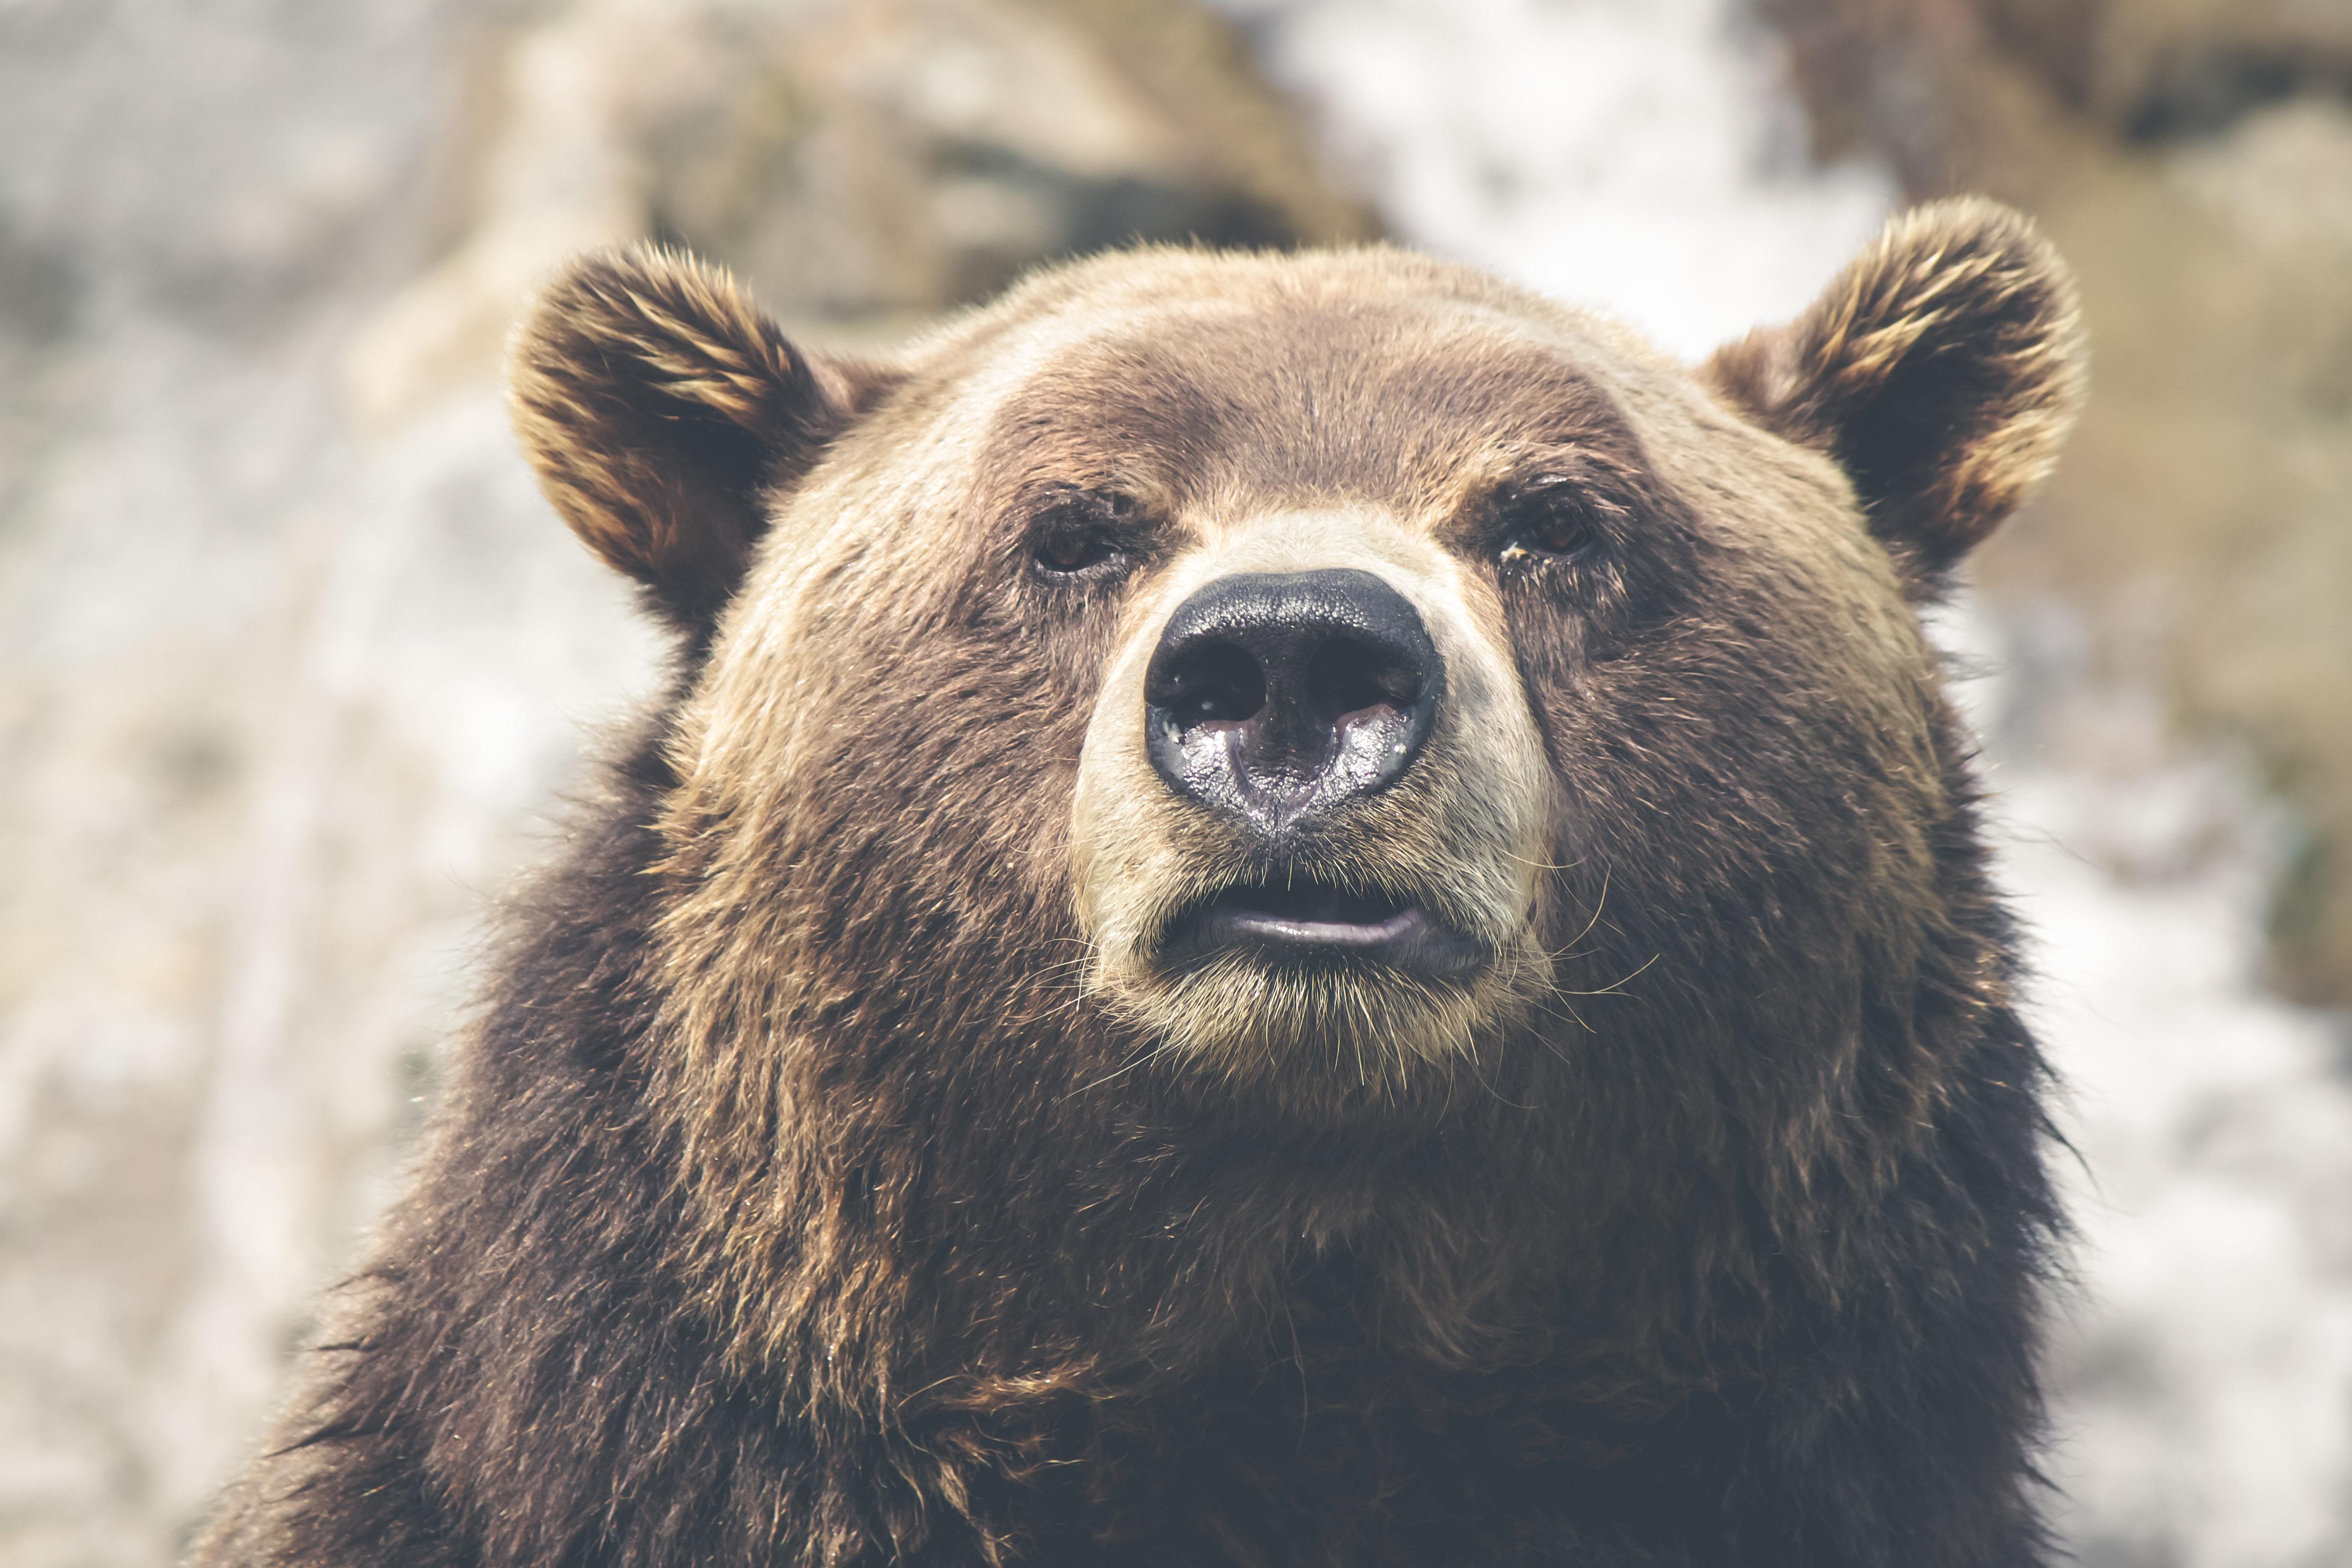
\includegraphics[width=\paperwidth,
                    height=\paperheight]{bear}
}                    
             
\subsection{Questions}

\begin{frame}[c]
\ \\ \ \\
\centering \Huge \textcolor{white}{\textbf{\forbold Questions? \newline Please make my day!}}

\end{frame}
\usebackgroundtemplate{}



\usebackgroundtemplate{
   \includegraphics[width=\paperwidth,
                    height=\paperheight]{sf}
}

\subsection{Thanks}


\begin{frame}[c]
%\setsansfont{Birds of Paradise}% the ! did not show
\setsansfont{SoupLeaf}
\ \\ \ \\
\centering \Huge \textcolor{AwesomeYellow}{\textbf{\forbold Thank You!}}
%\centering \Huge \textcolor{green}{\textbf{Thank You!}}
%{Thank You!}
\usebackgroundtemplate{}
\end{frame}

\end{document}
